% !TeX root = ./thesis.tex










%==============================
\chapter[Simulated predator attacks on flocks: a comparison of tactics]{Simulated\\ predator attacks on flocks:\\ a comparison of tactics}
\label{chap:alife}

\chapterAbstract[published={alife/Demšar_Lebar_Bajec_2014.pdf}, keywords={Bird, flock, artificial life, boid, fuzzy logic, predator}]{It is not exactly known why birds aggregate in coordinated flocks. The most common hypothesis proposes that the reason is protection from predators. Most of the currently developed examples of individual based predator-prey models assume predators are attracted to the centre of a highly coordinated flock. This proposed attraction of a predator to a flock would appear to be contradictory to an alternate hypothesis that flocks evolved as a protection against predation. In an attempt to resolve this apparent conflict, in this article we use a fuzzy individual based model to study three attack tactics (attack centre, attack nearest, attack isolated) and analyse the success of predation on two types of prey (social and individualistic). Our simulations revealed that social flocking (as opposed to individualistic behaviour) is the optimal anti-predatory response to predators attacking mainly isolated individuals.}

%-----
\section{Introduction}

The study of collective behaviour is a fascinating field that analyses how simple actions of an individual influence the complex global dynamics of a group. Aristotle once stated: ``The whole is greater than the sum of its parts.'' -- a statement that describes the essence of collective behaviour. Typical examples of collective behaviour are flocks of birds, schools of fish and swarms of insects; phenomena that can be easily observed in nature. Collective behaviour is also interesting because similar patterns emerge at smaller scales (cellular level) \cite{deisboeck2009collective,spector2003emergence}. Even though collective behaviour is a common sight, it is still surrounded by mystery \cite{lebarbajec2009organized}. Several different hypotheses in the literature suggest reasons why animals sometimes coalesce into organized groups. The most common one proposes that such groups may function as an effective defence against predators \cite{hart2005predator,krause2002living,lebarbajec2009organized,nishimura1997emergence}. This hypothesis is supported by evidence that animals in groups may benefit from an increased probability of detecting a predator \cite{galton1871gregariousness}, individuals in groups may reduce the amount of time spent for predator vigilance \cite{elgar1989predator,sadedin1998influence}, and an individual in a large group may have a lower probability of being attacked by a predator \cite{hamilton1971geometry}. Other hypotheses suggest that aggregating animals may benefit through higher mating efficiency, and more efficient foraging \cite{krebs1994behavioural}. Some studies claim that fish schools or bird flocks save energy because of hydrodynamic or aerodynamic benefits \cite{lissaman1970formation}, however the opinions on this matter are contradictory \cite{bill1976drag,partridge1979evidence,usherwood2011flying}. Our work focuses mainly on bird flocks, however some results can also be applied to fish schools, since they have some similarities in structure and behaviour, as they both operate in a three-dimensional world \cite{krause2002living}.

Bird flocks are among the most widely observed, yet least understood phenomena of collective behaviour, mostly because of the difficulty of obtaining field data, and with the exception of a few types of urban flocks, the unpredictability of the appearance of highly organized flocks in nature \cite{heppner1997threedimensional}. Two types of highly organized bird flocks emerge in nature -- luster flocks, demonstrated by pigeons and starlings, and line flocks, such as can be seen in groups of geese flying in a vee \cite{heppner1974avian}. Every evening, when birds that fly in organized groups return to their roosting areas, small flocks coalesce into giant cluster flocks, often numbering tens of thousands of birds. Birds may then perform complex aerial manoeuvres before finally settling in their roosts \cite{lebarbajec2009organized}. Such behaviour can often be seen every evening at the same place, so it might appear that birds flying in such flocks are actually attracting predators, and making it easy for them to attack the flock, which is counter intuitive with the idea that highly coordinated flocks evolved to reduce the impact of predation.

Complex flocking behaviour can emerge if individuals follow simple rules. In 1987, Reynolds \cite{reynolds1987flocks} published a ground-breaking paper that presented the first computer flocking animation (\emph{boids}). At the same time Heppner \& Grenander \cite{heppner1990stochastic} were working on a similar project in which they modelled birds' behaviour with stochastic nonlinear differential equations. In these two and most subsequent models equations govern the behaviour of the artificial animals (\emph{animats}). Our model uses fuzzy logic \cite{zadeh1965fuzzy} and fuzzy rule-based systems \cite{mamdani1974application,dasilva2008predator} to develop the behaviour of artificial animals, rather than equations.

Some current state-of-the-art models are in three dimensions and incorporate some simplified aerodynamics \cite{hildenbrandt2010selforganized}. To make an in-depth study of shapes and patterns that emerge within the flock during a predator attack a three-dimensional model would be required \cite{hemelrijk2011somecauses}, but for the purpose of our study a two-dimensional model suffices, since some researchers suggest that the dimensionality of the model minimally affects the results of the simulations \cite{huth1992simulation,huth1994simulation,kunz2012simulations} and others believe that models should be as simple as possible \cite{czirok2000collective}.

Various authors have upgraded the basic models to add additional functionalities. Moškon\etal, for example, used fuzzy logic to simulate the foraging behaviour of artificial birds \cite{moskon2007fuzzy}. There are also several models that implement predators. All of them are based on Reynolds' model and most of them use a predator that attacks the centre of the flock \cite{inada2002order,lee2006dynamics}. This predator attack tactic 
might be true for some species of real fish; a swordfish, for example, in nature typically attacks the centre of a prey school. In the first attack it disperses the school, and in the following attacks the swordfish focuses on the individual fish that become separated from the rest of the group \cite{stephens2003modelling}. Compared to birds, however fish may have better perception of the environment than birds because of the lateral line, and schooling might be used to confuse the lateral line of predators \cite{larsson2009possible}. Assuming that birds do not have a sense like the lateral line, avian predators in nature might not attack in such a fashion.

Others that studied predator-prey dynamics in collective behaviour mostly focused on a flock's response to the predator's attack. For example, Inada\etal focused on common escape patterns that emerge \cite{inada2002order}, while Lee\etal analysed how the size of the flocks changes during an attack \cite{lee2006dynamics}. 

In both cases the predator attacked the centre of the flock. With respect to the hypothesis that flocks form as a defensive mechanism, targeting the centre of the flock in hope of catching a prey might be viewed as a tactic based on pure luck. As already stated this attack tactic might not be used by avian predators, except maybe for the first attacks, where the goal might be to disperse the prey in order to prepare for other tactics whose positive outcome might be more probable. This research is not the first to propose different attack tactics; Nishimura \cite{nishimura2000studying,nishimura2002predator} was the first to study target selection mechanisms. The key differences of this research compared to Nishimura's studies are: 1) we use fuzzy logic; Nishimura used differential equations; 2) we model target selection through ``realistic'' visual perception; Nishimura defined the probability of a prey becoming a target through a mathematical equation that does not take into account the position of the predator relative to the flock, nor its orientation; 3) in our model the prey that ``sees'' the predator tries to escape; in Nishimura's model it does not; and 4) we study social versus individualistic prey behaviour; Nishimura studies ordered, partially disordered and fully disordered prey motion.

According to Nishimura's study \cite{nishimura2002predator} the best predator tactic is to attack a peripheral target and not the attack of an isolated target, as it can be observed in nature \cite{stephens2003modelling,ioannou2012predatory}. The reasons for this conclusion are two: a) the equation Nishimura uses for a predator targeting isolated prey (Nishimura's strategy S) will not select any target if none exists that has a large enough separation from the flock; and b) Nishimura's predator has perfect vision (\ie it is able to perceive all prey) and it can happen that the predator will select a target that is on the opposite side of the flock and therefore require a substantial amount of time to reach it. The first reason is unrealistic as from the three types of motion that Nishimura studies (\ie ordered, partially disordered, and fully disordered) ordered motion, a rare event in nature, is a clear favourite. The second is unrealistic as the selected target potentially might not be visible to the predator at all, due to occlusion.

The analysis of predator-prey pursuit is interesting not only from a biological perspective but also from the perspective of control theory \cite{nahin2012chases,wei2009pursuit}. The control theory approach could potentially represent an alternative, more mathematical approach to our study. However, we believe our fuzzy, individual based model with its differences from Nishimura's approach permit a simulation whose behaviour is closer to that of real birds.

%-----
\section{Methods}

The basis for our work is an existing fuzzy logic based bird flocking model made by Lebar Bajec\etal \cite{lebarbajec2005simulating}, called \emph{synflocks}. An artificial animal, an animat, can be described using three qualities: a) its \emph{perception} of the environment, b) its \emph{drives}, c) its \emph{action selection}. Perception acts as a filter of important information. Drives define desired actions that will fulfil the animal's needs. Action selection combines these actions and performs the appropriate locomotor response. Assuming the artificial universe constitutes only of artificial animals with no environmental factors like artificial trees, then an artificial animal's behaviour is dependent mostly on the position, direction, and speed of the neighbours it perceives.

The animats in our model use the basic Reynolds drives -- \emph{cohesion}, \emph{separation} and \emph{alignment} \cite{reynolds1987flocks}. Cohesion simulates attraction toward flock-mates and is modelled as the animat's tendency to fly towards distant flock-mates when there are none nearby. Separation is a drive which helps the animats to avoid collisions -- it forces an individual to fly away from flock-mates that are too close. With the third drive -- alignment -- ani\-mats synchronize their velocity (direction and speed of flight) with flock-mates. A visual representation of the drives can be seen in \figurename~\ref{figDrives}. In our model the drives are described with simple linguistic if-then rules. Fuzzy logic is used for the transformation of the rules into numerical values; the desired change in direction and speed of each individual animat. More precisely the if-then rules are used in a Mamdani fuzzy inference system \cite{mamdani1974application} (see supplementary material).

\begin{figure}
	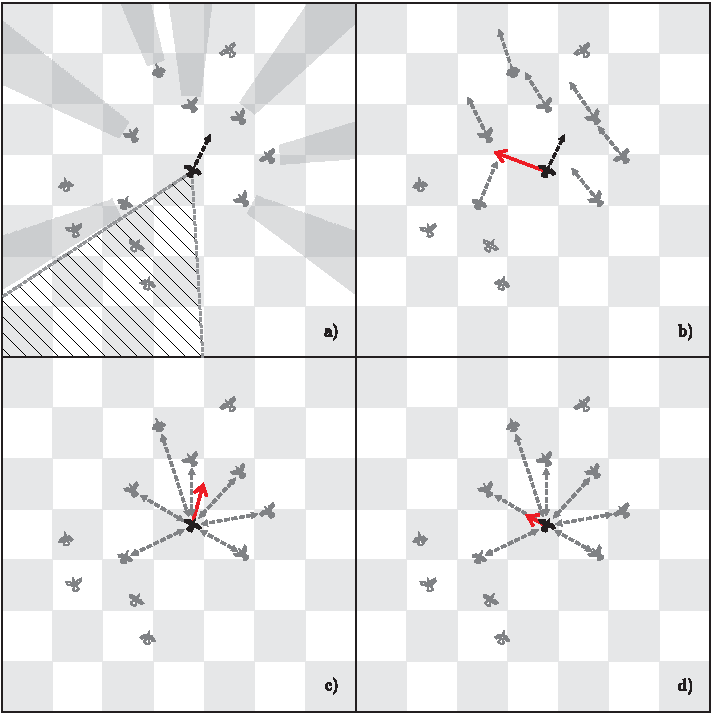
\includegraphics[width=\figurewidth]{alife/basicdrives}
	\caption{Perception of nearby neighbours (a). The black bird is the observed individual. The dark grey birds are the perceived nearby birds that influence the observed bird's behaviour. The white and outlined birds are either occluded by nearer birds (shaded areas), outside of the observed bird's field of vision (dashed area) or outside the number-limited range. Red arrows represent the resulting force vectors of the three basic drives -- lignment (b), cohesion (c), separation (d). The black bird is the observed individual, the dark grey birds are the influencing neighbours.}
	\label{figDrives}
\end{figure}

The original Reynolds' model and most existing models are based on metric distance. In these models every animat within a limited radius influences the behaviour of the observed animat; if an animat is outside that radius it does not have any influence on the observed individual. Nevertheless, recent research \cite{ballerini2008interaction,ballerini2008empirical} suggests that in nature only around seven nearest neighbours influence an individual. As this technique is already gaining support in current state-of-the-art models \cite{hildenbrandt2010selforganized}, we use a number-limited neighbourhood (topological distance) instead of a radius-limited neighbourhood (metric distance) as well. In models based on topological distance, only a fixed number of nearest animats is influential, regardless of their distance.

Our model uses topological distance and concentrates on vision as the principal means of neighbourhood perception. Our animat's field of vision is \ang{300} wide, with a blind angle of \ang{60} directly behind it. Most current models presume that birds have ``perfect'' vision and do not account for the occlusion of distant birds due to other birds flying in the flock. Yet a recent study by Kunz\etal \cite{kunz2012simulations} shows that obstruction of vision increases the realism of simulations. Our model thus takes into account only seven visible (non-occluded) nearby animats (see \figurename~\ref{figDrives}).

Predator and prey behaviours in our study are based on rules extracted from relevant theoretical literature and field observations. We modelled our simulations after a common scenario, where a Peregrine Falcon (\emph{Falco peregrinus}) is attacking a flock of European Starlings (\emph{Sturnus vulgaris}). In horizontal flight, the most economical flight speed (as to the amount of energy spent for flight propulsion) is around 60\% of the bird's maximum speed \cite{tennekes2009simple}. Let us call this speed the \emph{optimal cruising speed}. The optimal cruising speed of European Starling is \mps{11} and the optimal cruising speed of a Peregrine Falcon is \mps{13} \cite{tennekes2009simple}. In accordance to these values we set the maximum speed of our prey animat to \mps{18}, and the maximum speed of our predator animat to \mps{22}. Note that we presumed that the Peregrine Falcon was not hunting by using its characteristic hunting stoop (high speed dive), when it can reach speeds up to \mps{157} \cite{tucker1998gliding}. The minimum flight speed, in nature and in our model, is around 40\% of maximum flight speed \cite{tennekes2009simple}, which results in \mps{7.2} for prey animats and \mps{8.8} for the predator animat. To define the predator-prey relationship we introduced three additional drives -- \emph{hide}, \emph{seek}, and \emph{regulate speed}. The prey's behaviour is governed by the three basic drives (cohesion, separation, and alignment), and in addition hide, and regulate speed (see supplementary material for their explanation). The hide drive helps the prey to survive, as it forces it fly away from the attacking predator; it was tuned so that the direction of the prey's escape matches field observations by Handegard\etal \cite{handegard2012dynamics}. Regulate speed is only active when the hide drive is inactive -- when the predator is hidden from the prey's sight. This drive encourages prey to fly with their optimal cruising speed. The predator's behaviour is guided only by the seek drive (see supplementary material for its detailed explanation). With the seek drive the predator tries to catch the selected target.

\begin{figure}
	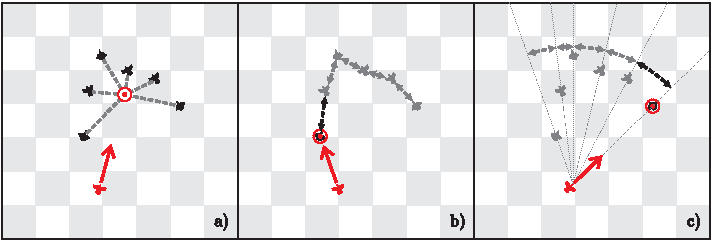
\includegraphics[width=\figurewidth]{alife/strategies}
	\infigurecaption{(a) the predator attacks the centre of the seven perceived prey, (b) the predator attacks the nearest of the seven perceived prey, (c) the predator attacks the most isolated of the seven perceived prey. The red bird is the predator and the red arrow represents the resulting force vector of the predator's seek drive.}	
	\caption{The three attack tactics.}
	\label{figStrategies}
\end{figure}

We implemented three different attack tactics (see \figurename~~\ref{figStrategies}). In our first tactic the predator attacks the centre point of the seven perceived prey. This mimics the tactic in which a predator attacks the centre of the flock in hope of hitting a target, but takes into account the limited amount of information available -- distance, relative position, difference in speed, and difference in heading of the perceived artificial animals.

In the second tactic, the predator attacks the nearest of the seven perceived prey. The nearest prey might be the one that is also the fastest to reach therefore making it a logical target for a predator. If a real predator chooses its prey in such a fashion then flocking might work as a mechanism to reduce an individuals' domain of danger \cite{hamilton1971geometry}. The domain of danger is defined as the area in which the observed individual is the predator's nearest neighbour. Obviously the average value of the domain of danger decreases if the number of birds in the flock increases, thus favouring tight highly organized flocks. By reducing the domain of danger an individual lowers the probability of being attacked by the predator, thus possibly increasing its chances of survival.

A predator using the third tactic attacks the most isolated of the seven perceived prey. In our study the most isolated prey is the one that has the largest \emph{angular distance} to its nearest neighbour. We defined angular distance as the angle between a potential target and its nearest neighbour -- from the predator's viewpoint. From a predator's viewpoint, isolated prey appear to have a large domain of danger because they are the most separated from the rest of the perceived prey. From the predator's perspective they would require the largest amount of time to decrease their domain of danger; time that is available to the predator to catch them. If we presume that flocking is indeed a protection mechanism, we can assume that the most isolated bird is the one that is the most vulnerable, making it a logical target for a predator.

%-----
\section{Results and discussion}

To recapitulate, the predator in our model uses one of the following three attack tactics: 1) \emph{attack centre} (\ie attack the centre point of the seven perceived prey), 2) \emph{attack nearest} (\ie attack the nearest of the seven perceived prey), 3) \emph{attack isolated} (\ie attack the most isolated, from the predator's point of view, of the seven perceived prey). In addition to escaping predator attacks and regulating their flight speed the prey can exhibit two types of behaviour: 1) \emph{social} behaviour (\ie prey obey the cohesion, separation, and alignment drives) or 2) \emph{individualistic} behaviour (\ie prey ignore the cohesion and alignment drives, but obey the separation drive to avoid collisions). In total this gives 6 combinations, through which we wished to answer the following questions: 1) what is the optimal predator tactic given a certain prey behaviour, 2) what is the optimal prey behaviour given a certain predator tactic.

\begin{figure}
	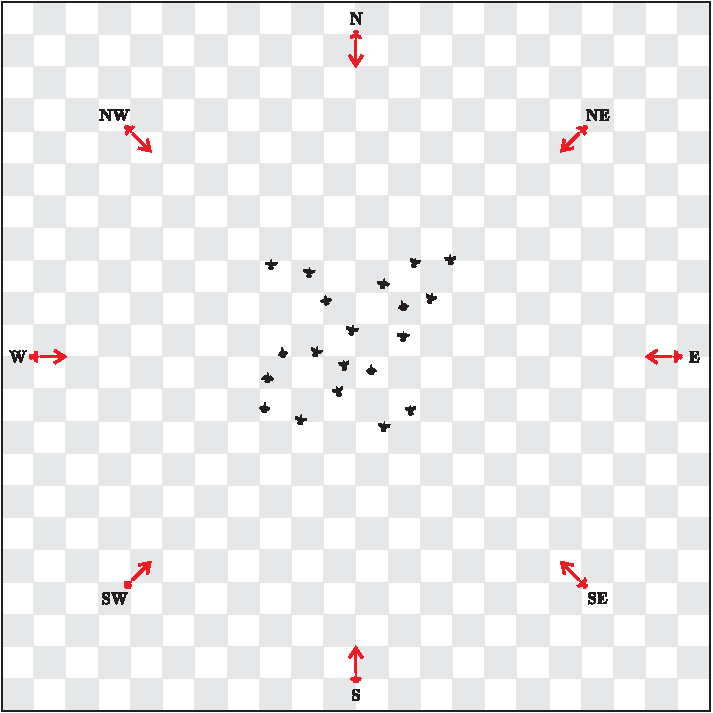
\includegraphics[width=\figurewidth]{alife/bearings}
	\caption{One of the starting configurations along with eight bearings of the predator's attack.}
	\label{figBearings}
\end{figure}

To provide answers to these questions we ran simulations where small cluster flocks consisting of 20, 40 or 60 social or individualistic prey were attacked by a predator from eight different bearings, relative to the flock. One of the starting configurations along with the eight bearings can be seen in \figurename~\ref{figBearings}. The different bearings were used to eliminate any dependency of the simulation's results on the predator's bearing (\eg a head on attack vs an attack from behind). This gives a total of 432 simulations (72 per configuration; selected predator attack tactic and prey behaviour). Each simulation was ran for 900 steps (frames) -- 30 seconds in our visualizations. We measured the time the predator needed to catch a prey. If the predator failed to catch the prey, the time-to-catch was set to 900 frames. The histograms of the time-to-catch for all simulations can be seen in \figurename~\ref{figHistograms}, with a more in depth discussion given in the following subsections.

\begin{figure}
	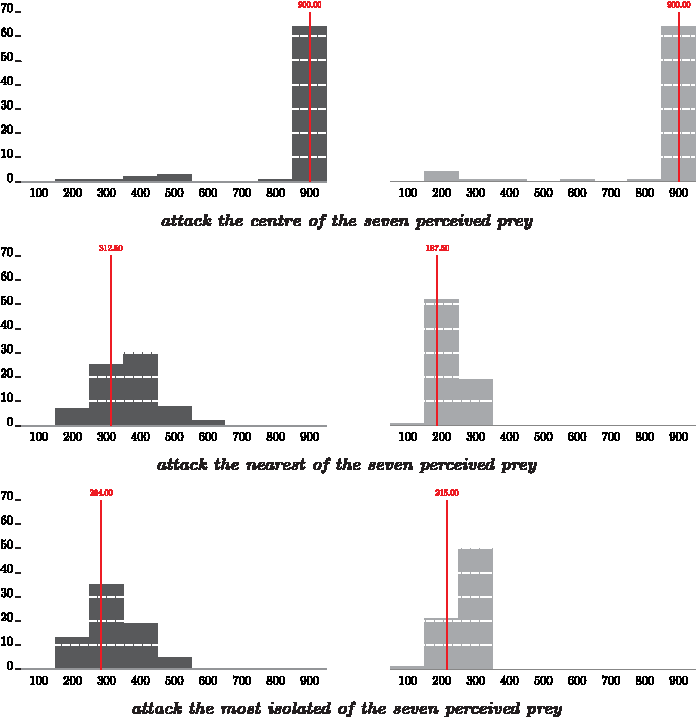
\includegraphics[width=\figurewidth]{alife/histograms}
	\caption{The influence of the predator's attack tactic and prey's behaviour on survivability of prey. Presented are six histograms of the predator's time-to-catch in corresponding simulation runs ($n=72$). Dark grey histograms present the time-to-catch in simulations with social prey, whereas light grey histograms present the time-to-catch in simulations with individualistic prey (cohesion and alignment drives not used). Red lines present the corresponding median time-to-catch.}
	\label{figHistograms}
\end{figure}

%-----
\subsection{Optimal predator tactic}

Our simulations suggest that the best tactic for a predator attacking flocks of social prey is the attack isolated tactic (\ttest{3.01}{142}{0.003}). It would appear that isolated prey benefit the least from the advantages of flocking. On average the predator needed \num{279.74} frames (\SD{72.29}) to catch an isolated prey. The predator whose tactic was to attack the nearest prey, needed \num{316.74} frames (\SD{75.76}) to catch its target, and the one, whose tactic was attack the centre of the seven perceived prey, needed \num{845.08} frames (\SD{165.04}).

With individualistic prey the best tactic for the predator is the attack nearest tactic (\ttest[<]{5.12}{140}{0.0001}). This finding makes sense, since the predator will get to the nearest prey faster than to those that are farther away. Predators that used this, attack nearest, tactic needed, on average, \num{177.31} frames (\SD{33.95}) to catch a prey. Predators that attacked isolated prey caught a prey in \num{208.06} frames (\SD{38.04}). The attack centre tactic proved to be the worst as the predator required \num{832.97} frames (\SD{198.89}) to catch a prey.

The predator that used the attack centre tactic was, in most cases, not successful. In other words it did not catch a prey in the 900 frames for which we ran the simulations (regardless if the prey was social or non-social). Thus the attack centre tactic proved to be the worst tactic regardless of the prey's behaviour.

As for the predator's best tactic overall, regardless of the prey's social or individualistic behaviour, no difference was found between the two most successful tactics, attack nearest and attack isolated (\ttest{0.34}{264}{0.73}).

%-----
\subsection{Optimal prey behaviour}

When the predator used the attack centre tactic no difference was found for the average time-to-catch between social and individualistic prey (\ttest{0.39}{137}{0.69}). In both cases the predator was rarely successful, which is a direct result of the predator's tactic that is based on pure luck.

With predators, whose tactic actually tries to optimize the chance of a positive result, however, the average time-to-catch is higher when prey behaviour is social than when prey behaviour is individualistic, more so when the predator targets the nearest prey (\ttest[<]{14.25}{98}{0.0001}) than when the predator uses the attack isolated tactic (\ttest[<]{7.42}{108}{0.0001}).

The best tactic for prey attacked by a predator appears to be social behaviour.

%-----
\subsection{Biological relevance}

Sonar fine-scale tracking of interactions among predatory fish and their schooling prey performed by Handegard\etal \cite{handegard2012dynamics} suggests that the most successful predators attack from behind. In our simulations, when the predator attacked from the side or front, the prey always managed to escape the initial attack. The predator was successful in one of the successive attacks that occurred from behind. Attacks from behind appear to be much more successful than other strategies as in some cases, when the predator attacked from behind, his initial attack was already fruitful. An example of the corresponding chase and escape paths in the case of a single predator attacking a single prey is presented in \figurename~\ref{figPaths}.

\begin{figure}
	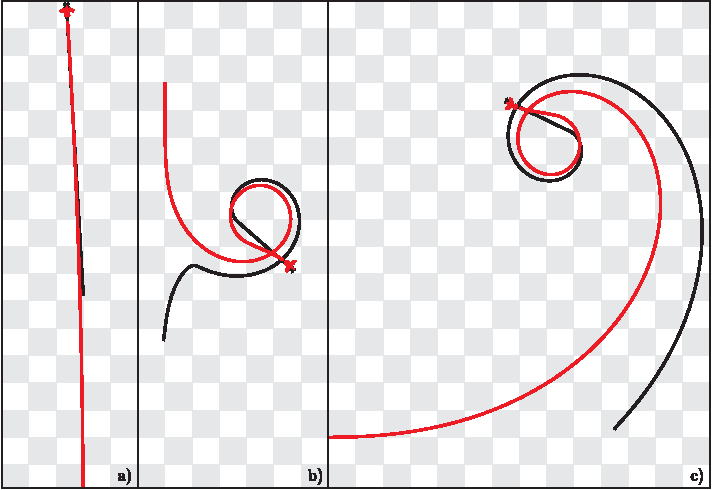
\includegraphics[width=\figurewidth]{alife/paths}
	\caption{Predator attacking a single prey from three main directions: (a) behind, (b) head on, (c) side.}
	\label{figPaths}
\end{figure}

In 1983, Pitcher and Wyche \cite{pitcher1983predator} defined several escape patterns. In our simulations, when the predator attacks the centre point of the seven perceived prey, prey show similar escape patterns as in nature and existing fish school models. Indeed we managed to spot three of the escape patterns defined by Pitcher \& Wyche \cite{pitcher1983predator}: \emph{herd}, \emph{split}, and \emph{fountain}. The herd pattern can be seen at the beginning of a predator approach. The herd pattern then morphs into either split or fountain. Split occurs when a large flock is divided into smaller ones. A typical characteristic of the fountain pattern is that the split flock rejoins behind the predator. These patterns can be seen in \figurename~\ref{figPatternsPhases}.

\begin{figure}
	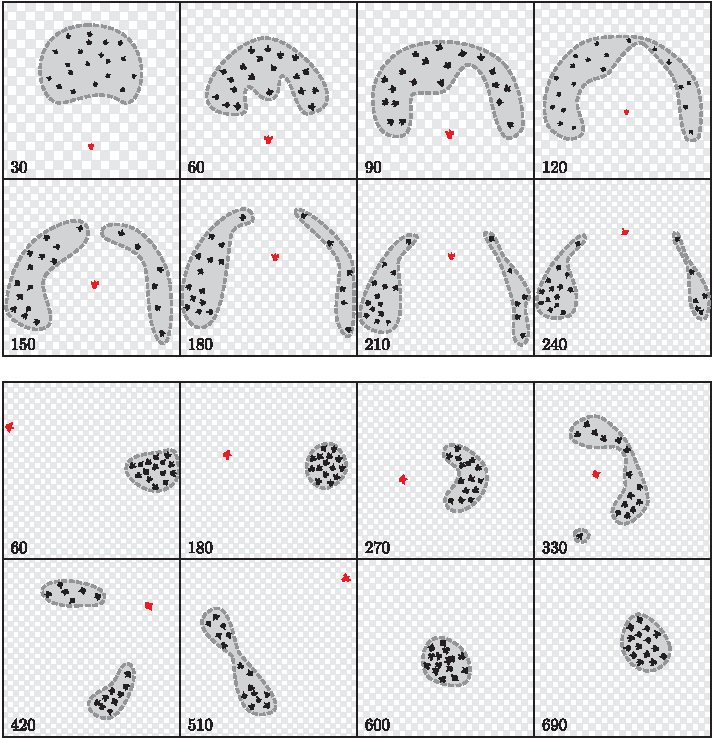
\includegraphics[width=\figurewidth]{alife/patternsPhases}
	\caption{Three common patterns in the artificial flock's response to a predator attack: (above) from \emph{herd} (frames 30--120) to \emph{split} (frames 120--240), (below) from \emph{herd} (frames 60--330) to \emph{fountain} (frames 330--510). In the below snapshots one can also notice the phases in the flock's response: before attack (frame 60), \emph{compression} (frames 60--180 and 510--600), \emph{expansion} (frames 270--510) and \emph{relaxation} (frames 600--690). The red bird is the predator, black birds represent prey. For the sake of clarity the birds were scaled by 200\% (above) and 300\% (below).}
	\label{figPatternsPhases}
\end{figure}

A more quantifiable measure was defined by Lee\etal \cite{lee2006dynamics}, who defined three phases that can be seen in artificial flocks during a predator attack -- \emph{compression}, \emph{expansion} and \emph{relaxation} (\figurename~\ref{figPatternsPhases}). In the first phase of an attack the flock's size decreases; this phase is called compression. In the second phase -- expansion -- prey try to move away from the predator. By doing this, the flock's size increases. In the last phase prey try to regroup, so the flock's size again decreases. This last phase is called relaxation. 

The three phases can easily be observed by tracing the artificial flock's \emph{flock size}, as defined by Lee\etal \cite{lee2006dynamics}:
%
\begin{equation}
\sigma = \sqrt{\frac{\sum_{i=1}^{N}{r_{i}^{2}}}{N}},
\end{equation}
%
where $r_i$ is the distance from the centre of the flock to the $i$-th individual, and $N$ is the total number of animats in the flock. All of our simulations showed a similar response of the artificial flock to a predator's attack. \figurename~\ref{figSizeChart} visualizes how, in our simulations, the flock size changes through time, both when the artificial flock is under threat from the predator and when there is no predator nearby. The flock size is measured in body lengths, one body length equals 20 centimetres, which is the size of a European Starling.

\begin{figure}
	\vskip3pt
	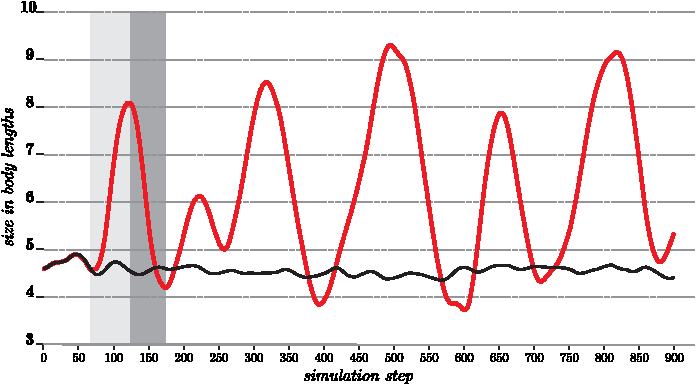
\includegraphics[width=\figurewidth]{alife/sizeChart}
	\infigurecaption{The black line shows the flock size when there is no predator nearby. The red line shows the flock size when the flock is under predator attack.}
	\caption{Plot of the flock size of an artificial flock consisting 20 animats. A clear example of flock expansion is marked with a light grey background, and dark grey is used to mark an example of flock compression. As predator attacks occur one after the other there is no clear example of flock relaxation.}
	\label{figSizeChart}
\end{figure}

%-----
\section{Conclusion}

Our simulations show that the least successful predator is the one that attacks the centre of the flock. They suggest that with predators whose tactic tries to optimize the chance of a positive outcome, social behaviour is more advantageous than individualistic behaviour, which strengthens our belief in the hypothesis that cluster flocking can be a mechanism for protection from predators. 

The behaviour of our artificial flocks appears to be comparable with that seen in flocks in nature. The average distance from nearest neighbour is around four body lengths (one body length equals 20 centimetres) \cite{ballerini2008empirical,major1978three,pomeroy1992structure}, the response of an artificial flock to a predator attack is similar to field observations \cite{lee2006dynamics}, and similar escape patterns emerge as in nature \cite{pitcher1983predator}. Our results also shows that the most successful predators attack from behind \cite{handegard2012dynamics}, and seek isolated targets \cite{ioannou2012predatory}. 

Our results seem to suggest that cluster flocking around a roost is paradoxical because although its structure might provide some protection against a predator attack, its very existence invites a predator attack, and at least in nature, there are always isolated individuals that can be picked off. It suggests also that at least in some circumstances, which may or may not be common in nature, tight cluster flocking can be of benefit to the flock as a whole, although it does not provide absolute protection to individuals in the flock.

%-----
\chapterAcknowledgements{We sincerely thank Frank H. Heppner of the University of Rhode Island and Maja Lebar Bajec for reading early drafts of the manuscript. Our gratitude also goes to Gregor Šega and Aleksandar Jurišić, who revised the statistical analysis of our results. This work was funded in part by the Slovenian Research Agency (ARRS) through the Pervasive Computing research programme (P2-0395).}

%=====
\begin{subappendices}

%-----
\section{Supplementary material}

In our model the animat is defined as a three stage process \cite{lebarbajec2005fuzzy}: perception, drives, action selection. For each animat the perception stage extrapolates data about the universe (other animats) that is available to the observed animat. In the drives stage, based on these data, a set of actions is computed that would fulfil individual needs of the modelled artificial animal. The action selection stage merges the actions and executes the locomotor response, thus changing the state of the universe.

%-----
\subsection{Perception}

In our model the universe consists of animats only; the universe is in essence a list of animats. To extrapolate data about the universe, as a first step, the observed animat is removed from this list, and the animats remaining in the list sorted based on their distance from the observed animat. Animats hidden by those that are closer to the observed animat or outside its field of view are then filtered out. The nearest seven animats remaining in the list provide the data about the universe. Only information about the relative position (\ie angular offset with respect to the observed animat's heading), distance, speed difference, and heading difference is passed on to the next stage.

Our approach differs from other existing models of number-limited neighbourhood (topological distance) \cite{ballerini2008interaction} in that it always takes into account a fixed number of nearest neighbours. Other models typically implement the number-limited neighbourhood as a \emph{variable} radius-limited neighbourhood \cite{hemelrijk2011somecauses}. In a variable radius-limited neighbourhood the observed animat will increase its radius of perception, if in the previous step it perceived less than the specified number of animats, and decrease it if in the previous step it perceived more than the specified number of animats. This approach in truth varies the number of perceived animats on every step of the simulation, but limits it to the specified number. The principal reason this approach is taken is probably the speed of computation. Its drawback is that the observed animat could potentially perceive all of the other animats, provided these were distributed so that they were all at the same distance from the observed animat.

The number of objects that can be stored in working memory in humans and other mammals is small, 4--7 \cite{ballerini2008interaction,engle1999individual}. The \emph{hippocampus}, the structure in the brain primarily responsible for working memory, is generally similar in birds and mammals \cite{sherry1989hippocampus}. Our use of seven nearest animats in the perceptual world of the prey and predator is thus based on research on working memory. In addition once the predator selects it target, in our model, it filters out all other potential prey, mimicking selective attention \cite{wiederman2012selective}.

%-----
\subsection{Drives}
The drives that result in actions that would fulfil the animat's individual needs are modelled using Mamdani fuzzy rules \cite{mamdani1974application}. For a detailed description of the cohesion, separation, and alignment drives, as well as a brief explanation of how a specific action is computed, the reader is invited to refer to \cite{lebarbajec2005simulating}. An in-depth description is available in \cite{lebarbajec2005fuzzy}. 

The data extrapolated in the previous stage are fuzzified as singletons and used as inputs for the fuzzy rules. The fuzzy variables, membership functions, and control rules for the hide drive can be seen in \figurename~\ref{figHide}. \figurename~\ref{figRegulateSpeed} presents the regulate speed drive, and \figurename~\ref{figSeek} presents the seek drive.\footnote{On the membership function charts that describe speed the value $1$ represents the appropriate maximum speed (predator's or prey's) while $-1$ represents the negative value of the appropriate maximum speed. While these are the desired changes in speed, the action selection stage ensures that the current speed of the observed individual never falls under the appropriate minimum speed (predator's or prey's).} The fuzzy rules are evaluated per individual perceived animat and the fuzzy outputs aggregated. 

\begin{figure}
	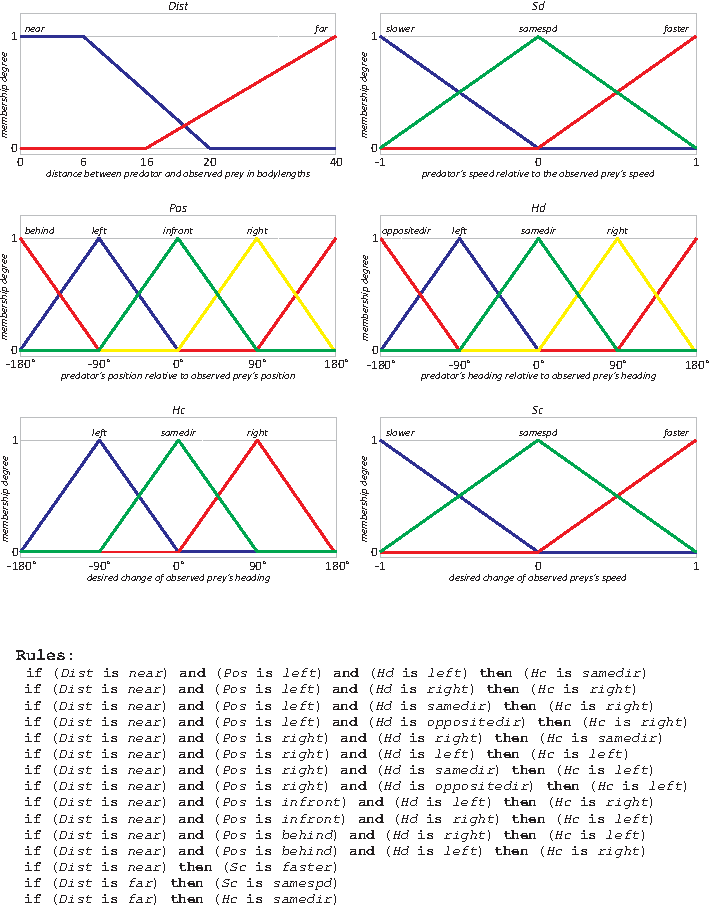
\includegraphics[width=\figurewidth]{alife/hide}
	\caption{Detailed description of the hide drive.}
	\label{figHide}
\end{figure}

\begin{figure}
	\parbox[c][.33\textheight]{\figurewidth}{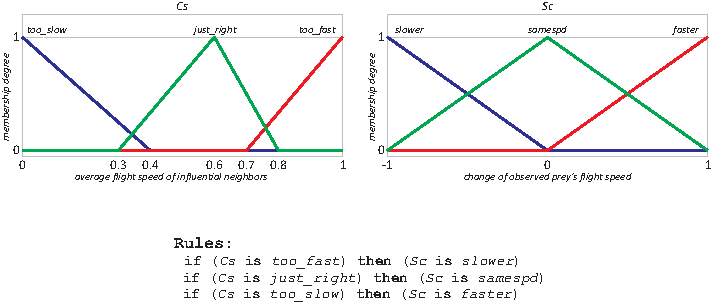
\includegraphics[width=\figurewidth]{alife/regulateSpeed}}
	\caption{Detailed description of the regulate speed drive.}
	\label{figRegulateSpeed}
\end{figure}

\begin{figure}
	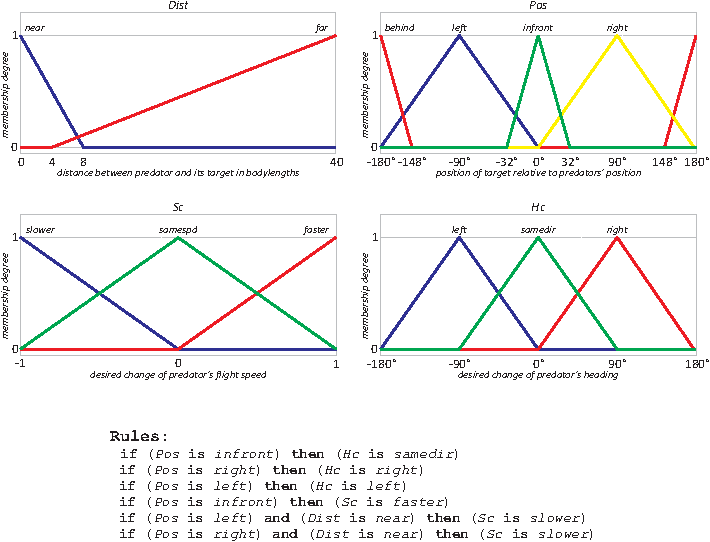
\includegraphics[width=\figurewidth]{alife/seek}
	\caption{Detailed description of the seek drive.}
	\label{figSeek}
\end{figure}

The fuzzy outputs are then defuzzified and a force vector computed. This force vector represents the action that will fulfil the individual need. It gives the direction and magnitude of the individual drive (the desired change in speed and direction). 

%-----
\subsection{Action selection}
In the action selection stage the force vectors resulting from individual drives are merged together and a resulting force vector computed. The merging is achieved through a simple weighted sum of the individual force vectors. The resulting force vector is interpreted as a Newtonian force based on which the observed animat's speed, heading and position are updated.

%-----
\subsection{Parameter values}
All of our model's parameters were either extrapolated from relevant theoretical literature (\eg speed, field of view, etc.) or tuned (\eg fuzzy membership functions, action selection mixing weights, etc.) so that the resemblance of the displayed behaviour to that observed in nature was visually as close as possible. For example, the action selection mixing weights have been configured so that the simulations visually resemble (as close as possible) field observations of flocking behaviour. In the prey's case these were (5, 5, 3, 4 and 1) for cohesion, separation, alignment, hide and regulate speed respectively. \tablename~\ref{table:parameters} presents all of the remaining parameters of the model. 

\begin{table}
	\caption{Default parameter values.}
	\label{table:parameters}
	\begin{tabular}{l l l}
		\toprule
		Parameter & Description & Default value \\ [0.5ex]
		\midrule 
		$\Delta t$ & Time step & 1 frame (\vfrac{1}{30}\,\si{\second}) \\
		$T$ & Maximum length of one simulation & 900 frames (\SI{30}{\second}) \\
		$v_\textnormal{aM}$ & Maximum speed of the predator animat & \mps{22} \\
		$v_\textnormal{am}$ & Minimum speed of the predator animat & \mps{8.8} \\
		$v_\textnormal{pM}$ & Maximum speed of prey animats & \mps{18} \\
		$v_\textnormal{pm}$ & Minimum speed of prey animats & \mps{7.2} \\
		$\varphi$ & Animat field of view & \ang{300} \\
		$n$ & Number of influential nearest neighbours & 7 \\
		$w_\textnormal{c}$ & Weight for cohesion drive & 5 \\
		$w_\textnormal{s}$ & Weight for separation drive & 5 \\
		$w_\textnormal{a}$ & Weight for alignment drive & 3 \\
		$w_\textnormal{e}$ & Weight for hide drive & 4 \\
		$w_\textnormal{rs}$ & Weight for regulate speed drive & 1 \\
		$w_\textnormal{h}$ & Weight for seek drive & 1 \\
		$l$ & Body length & \SI{0.2}{\metre} \\
		\midrule 
		& Fuzzification & singleton \\
		& Fuzzy conjunction & product \\
		& Fuzzy disjunction & probabilistic sum \\
		& Fuzzy implication & product \\
		& Fuzzy aggregation & probabilistic sum \\
		& Defuzzification & centrer of gravity \\
		\bottomrule 
	\end{tabular}
\end{table}

\end{subappendices}
